\chapter{Mekanisme Reaksi: Tahap Elementer dan Pendekatan}\label{ch:b1:elementary-steps}

Nitrogen monoksida, yang terbentuk di dalam mesin mobil dan oleh petir,
bergabung dengan oksigen udara: \ce{2NO + O2 -> 2NO2}. Jika diukur di
laboratorium, \omterm{def:b1:rate-laws:rate}{laju reaksi} ini sebanding dengan $[\ce{NO}]^2[\ce{O2}]$ ---
dan reaksi itu berlangsung \emph{lebih lambat} ketika gasnya dipanaskan.
Satu tumbukan tiga molekul dapat menjelaskan fakta pertama, tetapi tidak
pernah fakta kedua: setiap tumbukan menjadi lebih berenergi seiring
naiknya suhu. Penjelasannya ialah bahwa reaksi itu bukan satu peristiwa,
melainkan rangkaian peristiwa yang lebih sederhana, yaitu mekanismenya.
Bab ini mendefinisikan tahap-tahap elementer itu, \omterm{def:b1:elementary-steps:energy-profile}{profil energi} yang
dilaluinya, dan pendekatan-pendekatan yang mengubah sebuah mekanisme
menjadi \omterm{def:b1:rate-laws:order}{hukum laju}; bab ini ditutup dengan katalisis, seni membuka jalan
yang lebih mudah.

\begin{recall}
Buku 1 (kelas 12) memerikan \omterm{def:b1:elementary-steps:elementary-step}{mekanisme reaksi} sebagai rangkaian tahap yang
digambar dengan panah lengkung, dengan zat antara yang terbentuk dan
terpakai, dan \omterm{def:b1:elementary-steps:catalyst}{katalis} sebagai spesies yang mempercepat reaksi tanpa ikut
terpakai. \omterm{def:b1:rate-laws:order}{Hukum laju}, orde, dan \omterm{thm:b1:rate-laws:arrhenius}{hukum Arrhenius} didefinisikan pada
\cref{ch:b1:rate-laws}.
\end{recall}

\section{Tahap elementer}

\begin{definition}[Tahap elementer, molekularitas, mekanisme]\label{def:b1:elementary-steps:elementary-step}
\emph{Tahap elementer}\index{tahap elementer} adalah reaksi yang
berlangsung dalam satu peristiwa molekuler, persis seperti yang
dituliskan, tanpa zat antara apa pun. Banyaknya partikel yang bereaksi
dalam peristiwa itu adalah \emph{molekularitas}\index{molekularitas} tahap
itu: 1
(unimolekuler, sebuah penguraian atau penataan ulang), 2 (bimolekuler,
sebuah tumbukan), jarang 3.
\emph{Mekanisme reaksi}\index{mekanisme reaksi} adalah himpunan tahap elementer yang jumlahnya adalah reaksi
keseluruhan. Spesies yang terbentuk pada satu tahap dan terpakai pada
tahap sesudahnya, dan yang tidak muncul dalam persamaan keseluruhan,
adalah \emph{zat antara reaksi}\index{zat antara reaksi}.
\end{definition}

\begin{proposition}[Hukum laju sebuah tahap elementer]\label{prop:b1:elementary-steps:elementary-law}
\omterm{def:b1:elementary-steps:elementary-step}{Tahap elementer} mempunyai orde, dan orde-orde parsialnya sama dengan
koefisien stoikiometrinya: $\mathrm{A} \to \dots$ mempunyai $v = k[\mathrm{A}]$;
$\mathrm{A} + \mathrm{B} \to \dots$ mempunyai $v = k[\mathrm{A}][\mathrm{B}]$;
$2\,\mathrm{A} \to \dots$ mempunyai $v = k[\mathrm{A}]^2$. Kebalikannya
tidak benar: reaksi yang ordenya sama dengan koefisiennya belum tentu
elementer.
\end{proposition}

\begin{proof}[Penalaran]
Tahap bimolekuler terjadi ketika sebuah \ce{A} bertemu sebuah \ce{B};
banyaknya pertemuan semacam itu per satuan volume dan waktu sebanding
dengan banyaknya \ce{A} per satuan volume dan dengan banyaknya \ce{B},
sehingga sebanding dengan $[\ce{A}][\ce{B}]$. Tahap unimolekuler terjadi
pada setiap molekul dengan peluang tetap per satuan waktu, sehingga
lajunya sebanding dengan $[\ce{A}]$.
\end{proof}

\begin{remark}[Mengapa molekularitas jarang melebihi dua]\label{rem:b1:elementary-steps:termolecular}
Tiga partikel yang bertemu pada saat yang sama, masing-masing dengan
energi dan orientasi yang tepat, adalah peristiwa yang langka; reaksi
berorde total 3 hampir selalu merupakan hasil dua tahap bimolekuler yang
berurutan, seperti dalam soal akhir pekan.
\end{remark}

\section{Profil energi}

\begin{definition}[Koordinat reaksi, profil energi, keadaan transisi]\label{def:b1:elementary-steps:energy-profile}
Sepanjang sebuah \omterm{def:b1:elementary-steps:elementary-step}{tahap elementer}, atom-atom bergerak dari susunan
pereaksi ke susunan produk; variabel yang mengukur kemajuan ini (sebuah
panjang ikatan yang membesar, panjang ikatan lain yang mengecil) adalah
\emph{koordinat reaksi}\index{koordinat reaksi}. Grafik energi potensial
sistem sepanjang koordinat itu adalah
\emph{profil energi}\index{profil energi}. Maksimumnya adalah
\emph{keadaan transisi}\index{keadaan transisi}, sebuah susunan atom dengan ikatan-ikatan yang setengah
terbentuk dan setengah putus, yang tidak bertahan lebih lama daripada
satu getaran molekul dan tidak dapat diisolasi. Tinggi maksimum ini di
atas pereaksi adalah sawar energi tahap itu.
\end{definition}

\begin{omfigure}
\begin{tikzpicture}
\begin{axis}[omprofile, name=a,
  width=0.48\linewidth, height=5.4cm, xmin=0, xmax=10, ymin=-68, ymax=95,
  xlabel={koordinat reaksi}, ylabel={energi}]
\addplot[omDef, very thick] table[x=x, y=E] {figdata/out/bachelor-1-energy-profiles-one-step.dat};
\draw[dashed, black!40] (axis cs:0,0) -- (axis cs:10,0);
\draw[<->, omThm] (axis cs:5,0) -- (axis cs:5,79);
\node[omThm, anchor=west, font=\small] at (axis cs:5.1,30) {sawar};
\draw[<->, omProp] (axis cs:9.9,0) -- (axis cs:9.9,-40);
\node[omProp, anchor=east, font=\small] at (axis cs:9.8,-14) {$\Delta E$};
\node[anchor=south, font=\small] at (axis cs:5,81) {keadaan transisi};
\node[anchor=north west, font=\small] at (axis cs:0.15,-3) {pereaksi};
\node[anchor=north, font=\small] at (axis cs:8.6,-42) {produk};
\end{axis}
\begin{axis}[omprofile, at={(a.east)}, anchor=west, xshift=1.2cm,
  width=0.48\linewidth, height=5.4cm, xmin=0, xmax=10, ymin=-64, ymax=95,
  xlabel={koordinat reaksi}, ylabel={energi}]
\addplot[omDef, very thick] table[x=x, y=E] {figdata/out/bachelor-1-energy-profiles-two-step.dat};
\node[anchor=south, font=\small] at (axis cs:3,71) {KT 1};
\node[anchor=south, font=\small] at (axis cs:7,56) {KT 2};
\node[anchor=north, font=\small, align=center] at (axis cs:5,27) {zat\\antara};
\node[anchor=north west, font=\small] at (axis cs:0.15,-3) {pereaksi};
\node[anchor=north east, font=\small] at (axis cs:10,-43) {produk};
\end{axis}
\end{tikzpicture}

{\small Kiri: profil satu \omterm{def:b1:elementary-steps:elementary-step}{tahap elementer}, dengan sawarnya dan perubahan
energi reaksinya. Kanan: mekanisme dua tahap; zat antara terletak di
sebuah lembah di antara dua \omterm{def:b1:elementary-steps:energy-profile}{keadaan transisi} (KT). Energi-energinya
bersifat ilustratif.}
\end{omfigure}

\begin{proposition}[Sawar dan hukum Arrhenius]\label{prop:b1:elementary-steps:barrier}
\omterm{def:b1:rate-laws:activation-energy}{Energi aktivasi} sebuah \omterm{def:b1:elementary-steps:elementary-step}{tahap elementer} mendekati sawarnya: hanya
tumbukan yang membawa sedikitnya energi itu yang mencapai \omterm{def:b1:elementary-steps:energy-profile}{keadaan
transisi}. Untuk arah maju dan arah balik sebuah tahap, $E_{a,+} -
E_{a,-} = \Delta E$, yaitu energi reaksi tahap itu.
\end{proposition}

\begin{proof}[Penalaran]
Tahap balik mendaki sawar yang sama dari sisi yang lain: tingginya, yang
diukur dari produk, melebihi tinggi sawar maju sebesar $-\Delta E$.
\end{proof}

\begin{proposition}[Postulat Hammond]\label{prop:b1:elementary-steps:hammond}
\omterm{def:b1:elementary-steps:energy-profile}{Keadaan transisi} sebuah \omterm{def:b1:elementary-steps:elementary-step}{tahap elementer} menyerupai, dalam struktur dan
energinya, spesies yang energinya lebih dekat dengannya: produk untuk
tahap yang sangat menanjak (endoterm), pereaksi untuk tahap yang sangat
menurun (eksoterm). Akibatnya, untuk tahap yang membentuk zat antara
berenergi tinggi, apa pun yang menstabilkan zat antara itu juga
menurunkan sawar yang menuju kepadanya.
\end{proposition}
\admitted

\section{Tahap penentu laju dan prakesetimbangan}

\begin{definition}[Tahap penentu laju]\label{def:b1:elementary-steps:rds}
Dalam rangkaian tahap,
\emph{tahap penentu laju}\index{tahap penentu laju} adalah tahap yang jauh lebih lambat daripada semua tahap lainnya;
laju keseluruhan sama dengan lajunya, dan tahap-tahap yang lebih cepat
menyesuaikan diri dengannya seperti mobil-mobil di sebuah jalan
mengikuti titik terlambatnya.
\end{definition}

\begin{definition}[Pendekatan prakesetimbangan]\label{def:b1:elementary-steps:pre-equilibrium}
Dalam \emph{pendekatan prakesetimbangan}\index{pendekatan prakesetimbangan},
sebuah tahap reversibel yang cepat yang mendahului \omterm{def:b1:elementary-steps:rds}{tahap penentu laju}
dianggap tetap berada dalam kesetimbangan sepanjang waktu:
konsentrasi-konsentrasi spesiesnya mematuhi tetapan kesetimbangannya
$K_1 = k_1/k_{-1}$.
\end{definition}

\begin{proposition}[Hukum laju dari prakesetimbangan]\label{prop:b1:elementary-steps:pre-equilibrium-law}
Untuk mekanisme
\[
  \mathrm{A} + \mathrm{B} \underset{k_{-1}}{\overset{k_1}{\rightleftharpoons}} \mathrm{I}
  \ \text{(cepat)}, \qquad
  \mathrm{I} + \mathrm{C} \xrightarrow{\ k_2\ } \mathrm{P} \ \text{(lambat)},
\]
lajunya $v = k_2K_1[\mathrm{A}][\mathrm{B}][\mathrm{C}]$, berorde total 3,
dengan tetapan semu $k = k_1k_2/k_{-1}$.
\end{proposition}

\begin{proof}
Lajunya adalah laju tahap yang lambat, $v = k_2[\mathrm{I}][\mathrm{C}]$.
Tahap pertama tetap dalam kesetimbangan: $k_1[\mathrm{A}][\mathrm{B}] =
k_{-1}[\mathrm{I}]$, sehingga $[\mathrm{I}] = K_1[\mathrm{A}][\mathrm{B}]$.
Substitusi menghasilkan hasil tersebut.
\end{proof}

\section{Pendekatan keadaan tunak}

\begin{theorem}[Reaksi orde satu berurutan]\label{thm:b1:elementary-steps:consecutive}
Untuk $\mathrm{A} \xrightarrow{k_1} \mathrm{B} \xrightarrow{k_2} \mathrm{C}$,
kedua tahapnya berorde 1, dengan $[\mathrm{A}] = a_0$ dan $[\mathrm{B}] =
[\mathrm{C}] = 0$ pada $t = 0$ dan $k_1 \ne k_2$:
\[
  [\mathrm{A}] = a_0\eu^{-k_1t}, \qquad
  [\mathrm{B}] = \frac{a_0k_1}{k_2 - k_1}\big(\eu^{-k_1t} - \eu^{-k_2t}\big),
  \qquad [\mathrm{C}] = a_0 - [\mathrm{A}] - [\mathrm{B}] .
\]
Zat antara melewati sebuah maksimum pada $t_{\max} = \dfrac{\ln(k_2/k_1)}
{k_2 - k_1}$.
\end{theorem}

\begin{proof}
$\dd[\mathrm{A}]/\dd t = -k_1[\mathrm{A}]$ menghasilkan $[\mathrm{A}]$. Lalu
$\dd[\mathrm{B}]/\dd t + k_2[\mathrm{B}] = k_1a_0\eu^{-k_1t}$, sebuah
persamaan linear orde satu: dengan mengalikannya dengan $\eu^{k_2t}$, $\frac{\dd}{\dd t}
\big([\mathrm{B}]\eu^{k_2t}\big) = k_1a_0\eu^{(k_2-k_1)t}$, yang
integralnya dari 0, ketika $[\mathrm{B}] = 0$, adalah $[\mathrm{B}]\eu^{k_2t} =
\frac{k_1a_0}{k_2-k_1}(\eu^{(k_2-k_1)t} - 1)$. Kekekalan materi menghasilkan
$[\mathrm{C}]$. Turunan $[\mathrm{B}]$ sama dengan nol ketika $k_1\eu^{-k_1t}
= k_2\eu^{-k_2t}$, yaitu pada $t_{\max}$.
\end{proof}

\begin{definition}[Pendekatan keadaan tunak]\label{def:b1:elementary-steps:qssa}
Dalam \emph{pendekatan keadaan tunak}\index{pendekatan keadaan tunak}
(atau keadaan kuasi-tunak), konsentrasi zat antara yang sangat reaktif,
yang terpakai jauh lebih cepat daripada terbentuknya, dianggap tetap dan
kecil sesudah masa induksi yang singkat: \omterm{def:b1:rate-laws:rate}{laju pembentukannya} sama dengan
laju pemakaiannya,
$\dd[\mathrm{I}]/\dd t \approx 0$.
\end{definition}

\begin{proposition}[Kapan keadaan tunak berlaku]\label{prop:b1:elementary-steps:qssa-justified}
Untuk $\mathrm{A} \to \mathrm{B} \to \mathrm{C}$ dengan $k_2 \gg k_1$:
sesudah waktu yang berorde $1/k_2$, $[\mathrm{B}] \approx k_1[\mathrm{A}]/k_2$ (yaitu
yang dihasilkan oleh $\dd[\mathrm{B}]/\dd t = 0$), $[\mathrm{B}]$ tetap kecil, dan
produk terbentuk dengan laju $\dd[\mathrm{C}]/\dd t \approx k_1[\mathrm{A}]$:
tahap pertama adalah \omterm{def:b1:elementary-steps:rds}{tahap penentu laju}.
\end{proposition}

\begin{proof}
Untuk $k_2 \gg k_1$ dan $t \gg 1/k_2$, $\eu^{-k_2t}$ dapat diabaikan
dibandingkan dengan $\eu^{-k_1t}$ dan $k_2 - k_1 \approx k_2$, sehingga
$[\mathrm{B}] \approx (a_0k_1/k_2)
\eu^{-k_1t} = k_1[\mathrm{A}]/k_2 \ll [\mathrm{A}]$. Maka
$\dd[\mathrm{C}]/\dd t = k_2[\mathrm{B}] \approx k_1[\mathrm{A}]$.
\end{proof}

\begin{omfigure}
\begin{tikzpicture}
\begin{axis}[name=s,
  width=0.48\linewidth, height=5.2cm, xmin=0, xmax=6, ymin=0, ymax=1.05,
  axis x line=bottom, axis y line=left,
  xlabel={$k_1t$}, ylabel={konsentrasi$/a_0$},
  title={$k_2 = 0.5\,k_1$}, title style={font=\small},
  tick label style={font=\small}, label style={font=\small}]
\addplot[omDef, thick] table[x=t, y=a] {figdata/out/bachelor-1-consecutive-reactions-slow.dat};
\addplot[omThm, thick] table[x=t, y=b] {figdata/out/bachelor-1-consecutive-reactions-slow.dat};
\addplot[omMeth, thick] table[x=t, y=c] {figdata/out/bachelor-1-consecutive-reactions-slow.dat};
\node[omDef, font=\small, anchor=west] at (axis cs:0.4,0.75) {A};
\node[omThm, font=\small, anchor=south] at (axis cs:1.39,0.51) {B};
\node[omMeth, font=\small, anchor=west] at (axis cs:4.5,0.75) {C};
\end{axis}
\begin{axis}[at={(s.east)}, anchor=west, xshift=1.2cm,
  width=0.48\linewidth, height=5.2cm, xmin=0, xmax=6, ymin=0, ymax=1.05,
  axis x line=bottom, axis y line=left,
  xlabel={$k_1t$}, ylabel={konsentrasi$/a_0$},
  title={$k_2 = 20\,k_1$}, title style={font=\small},
  tick label style={font=\small}, label style={font=\small}]
\addplot[omDef, thick] table[x=t, y=a] {figdata/out/bachelor-1-consecutive-reactions-fast.dat};
\addplot[omThm, thick] table[x=t, y=b] {figdata/out/bachelor-1-consecutive-reactions-fast.dat};
\addplot[omMeth, thick] table[x=t, y=c] {figdata/out/bachelor-1-consecutive-reactions-fast.dat};
\addplot[black, dashed] table[x=t, y=bss] {figdata/out/bachelor-1-consecutive-reactions-fast.dat};
\node[omDef, font=\small, anchor=west] at (axis cs:1.4,0.32) {A};
\node[omThm, font=\small, anchor=south west, align=left] at (axis cs:2,0.22) {B (keadaan tunak,\\putus-putus)};
\node[omMeth, font=\small, anchor=west] at (axis cs:4.5,0.85) {C};
\end{axis}
\end{tikzpicture}

{\small Reaksi berurutan $\mathrm{A} \to \mathrm{B} \to \mathrm{C}$.
Kiri: zat antara menumpuk dan mencapai puncak pada $k_1t = 1.39$. Kanan:
jika zat antara itu terpakai dua puluh kali lebih cepat daripada
terbentuknya, konsentrasinya tetap kecil dan mengikuti nilai keadaan
tunak $k_1[\mathrm{A}]/k_2$ (putus-putus) sesudah masa induksi yang
singkat.}
\end{omfigure}

\begin{method}[Hukum laju dari sebuah mekanisme]\label{met:b1:elementary-steps:rate-law}
Untuk menurunkan \omterm{def:b1:rate-laws:order}{hukum laju} sebuah mekanisme:
\begin{enumerate}
  \item tuliskan laju setiap \omterm{def:b1:elementary-steps:elementary-step}{tahap elementer} (\cref{prop:b1:elementary-steps:elementary-law});
  \item nyatakan laju keseluruhan sebagai \omterm{def:b1:rate-laws:rate}{laju pembentukan} sebuah produk
        (dibagi dengan koefisiennya);
  \item eliminasi setiap zat antara dengan \omterm{def:b1:elementary-steps:qssa}{pendekatan keadaan tunak}
        ($\dd[\mathrm{I}]/\dd t = 0$, sebuah persamaan aljabar) atau, jika
        sebuah kesetimbangan cepat mendahului tahap yang lambat, dengan
        tetapannya;
  \item sederhanakan pada limit-limit ketika satu suku dominan, lalu
        bandingkan dengan hukum eksperimen.
\end{enumerate}
\end{method}

\begin{example}[Reaksi yang dikatalisis asam]\label{ex:b1:elementary-steps:acid}
Untuk $\mathrm{S} + \ce{H3O+} \rightleftharpoons \mathrm{SH}^+ + \ce{H2O}$ (cepat,
tetapan $K_1$) yang diikuti $\mathrm{SH}^+ + \ce{H2O} \to \mathrm{P} + \ce{H3O+}$ (lambat,
$k_2$), lajunya $v = k_2[\mathrm{SH}^+] = k_2K_1[\mathrm{S}][\ce{H3O+}]$:
orde satu terhadap substrat dan terhadap asam, walaupun asamnya tidak
terpakai.
\end{example}

\section{Katalisis dan pengendalian selektivitas}

\begin{definition}[Katalis, katalisis homogen dan heterogen]\label{def:b1:elementary-steps:catalyst}
\emph{Katalis}\index{katalis} adalah spesies yang menaikkan laju sebuah
reaksi tanpa muncul dalam persamaan keseluruhannya: terpakai pada satu
tahap mekanisme, katalis itu dibentuk kembali pada tahap sesudahnya.
Dalam \emph{katalisis homogen}\index{katalisis homogen}, katalis berada
dalam \omterm{def:b1:extent-q-and-k:system}{fase} yang sama dengan pereaksi (asam terlarut, kompleks logam,
enzim); dalam \emph{katalisis heterogen}\index{katalisis heterogen},
katalis merupakan \omterm{def:b1:extent-q-and-k:system}{fase} tersendiri, biasanya padatan yang di permukaannya
reaksi berlangsung (platina, besi, zeolit).
\end{definition}

\begin{proposition}[Apa yang diubah katalis]\label{prop:b1:elementary-steps:catalysis}
\omterm{def:b1:elementary-steps:catalyst}{Katalis} menyediakan mekanisme baru yang sawarnya lebih rendah. \omterm{def:b1:elementary-steps:catalyst}{Katalis}
mempercepat reaksi maju dan reaksi balik dengan rasio yang sama, sehingga
tidak mengubah tetapan kesetimbangan, keadaan akhir, dan energi reaksi.
\end{proposition}

\begin{proof}
Untuk \omterm{def:b1:elementary-steps:elementary-step}{tahap elementer} dalam kesetimbangan, laju maju dan laju balik sama:
$k_+[\text{pereaksi}] = k_-[\text{produk}]$, sehingga $K = k_+/k_-$.
Untuk mekanisme apa pun dalam kesetimbangan, setiap tahap berada dalam
kesetimbangan (jika tidak, sebagian spesies akan terus berubah), dan $K$
adalah hasil kali rasio-rasio $k_+/k_-$ tahap-tahapnya. Jalan yang
dikatalisis mencapai keadaan akhir yang sama, dengan tetapan yang sama:
dengan faktor berapa pun ia mengalikan $k_+$, ia mengalikan $k_-$
dengan faktor yang sama.
\end{proof}

\begin{omfigure}
\begin{tikzpicture}
\begin{axis}[omprofile,
  width=0.62\linewidth, height=5.6cm, xmin=0, xmax=10, ymin=-45, ymax=115,
  xlabel={koordinat reaksi}, ylabel={energi}]
\addplot[black!60, very thick] table[x=x, y=E] {figdata/out/bachelor-1-energy-profiles-uncatalysed.dat};
\addplot[omMeth, very thick] table[x=x, y=E] {figdata/out/bachelor-1-energy-profiles-catalysed.dat};
\node[anchor=south, font=\small] at (axis cs:5,101) {tanpa katalis};
\node[omMeth, anchor=north, font=\small] at (axis cs:3.5,-6) {dengan katalis};
\draw[<->, omProp] (axis cs:10.4,0) -- (axis cs:10.4,-30);
\draw[dashed, black!40] (axis cs:0,0) -- (axis cs:10.6,0);
\node[omProp, anchor=west, font=\small] at (axis cs:10.5,-15) {$\Delta E$ tetap};
\end{axis}
\end{tikzpicture}

{\small \omterm{def:b1:elementary-steps:catalyst}{Katalis} membuka jalan dengan sawar yang lebih rendah (hijau),
sering kali dalam beberapa tahap; awal dan akhirnya, sehingga energi
reaksi dan kesetimbangannya, tetap sama.}
\end{omfigure}

\begin{omfigure}
\begin{tikzpicture}[font=\small, >={Stealth}]
  \node[draw=omMeth, rounded corners, fill=omMeth!10, minimum width=2.4cm] (c) at (0,1.6) {katalis};
  \node[draw=black!50, rounded corners, fill=black!5, minimum width=2.4cm] (i1) at (2.6,0) {kompleks 1};
  \node[draw=black!50, rounded corners, fill=black!5, minimum width=2.4cm] (i2) at (0,-1.6) {kompleks 2};
  \node[draw=black!50, rounded corners, fill=black!5, minimum width=2.4cm] (i3) at (-2.6,0) {kompleks 3};
  \draw[->, thick] (c) to[bend left=20] node[above right] {+ A} (i1);
  \draw[->, thick] (i1) to[bend left=20] node[below right] {+ B} (i2);
  \draw[->, thick] (i2) to[bend left=20] node[below left] {} (i3);
  \draw[->, thick] (i3) to[bend left=20] node[above left] {$-$ P} (c);
\end{tikzpicture}

{\small Sebuah siklus katalitik: \omterm{def:b1:elementary-steps:catalyst}{katalis} mengikat pereaksi A dan B secara
bergiliran, produk P dilepaskan, dan \omterm{def:b1:elementary-steps:catalyst}{katalis} dibentuk kembali untuk
memulai lagi. Siklus katalitik kompleks logam dipelajari dalam jilid
Tahun 2.}
\end{omfigure}

\begin{omfigure}
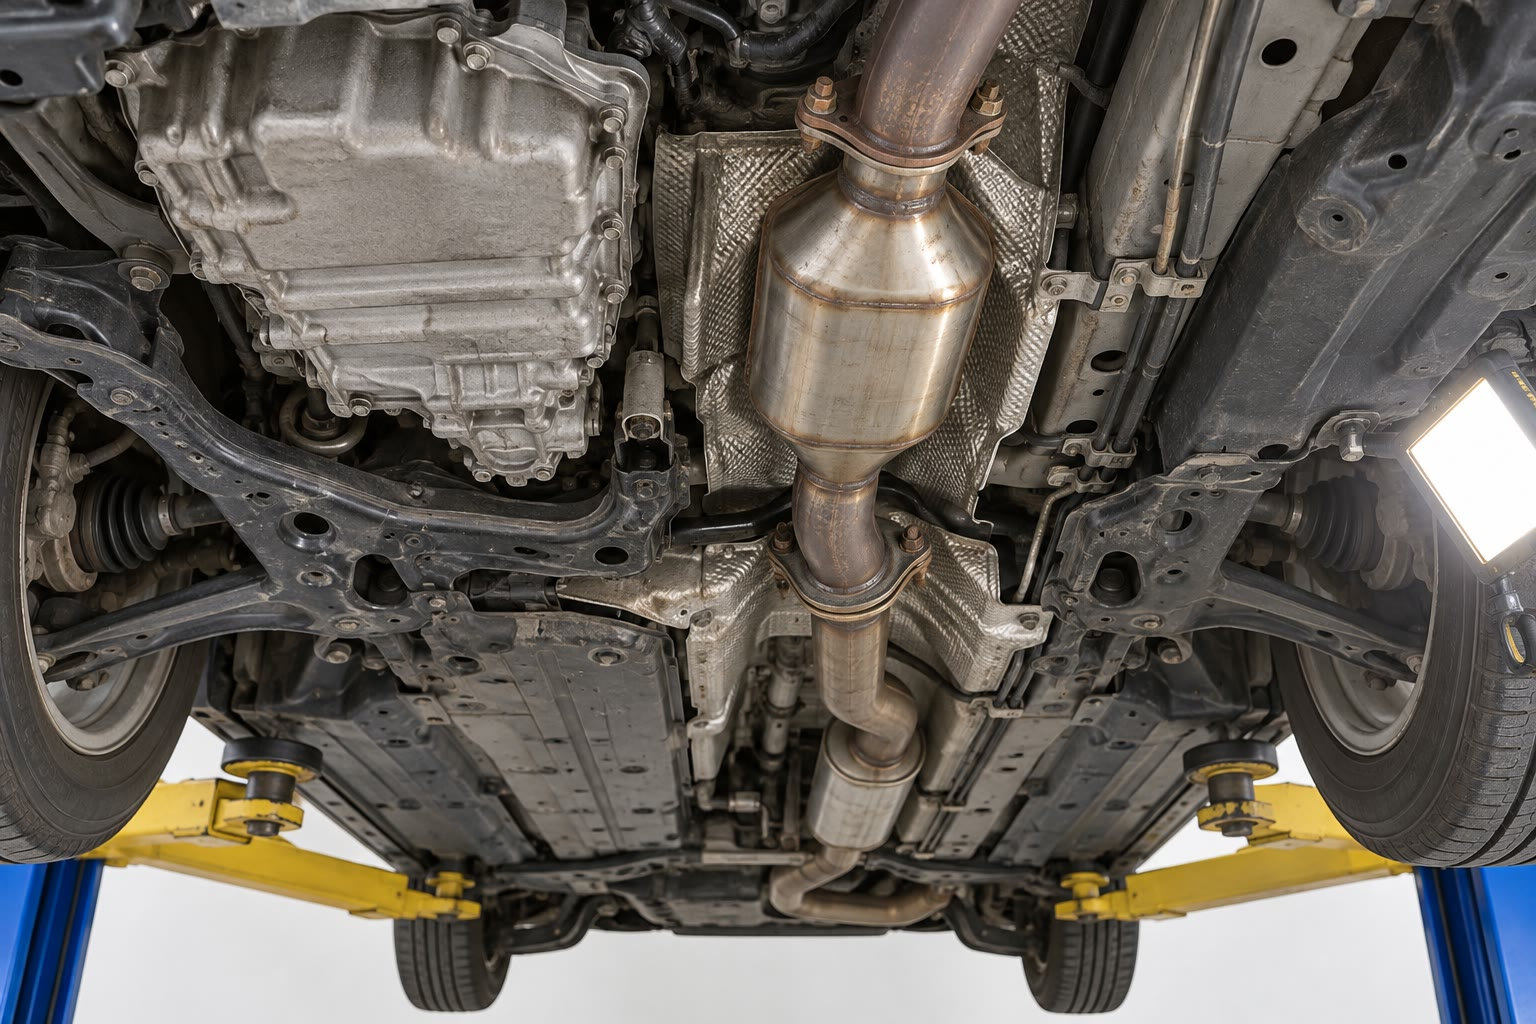
\includegraphics[width=0.5\linewidth]{images/book2/ai/b1-09-catalytic-converter.jpg}

{\small Bagian bawah sebuah mobil: tabung pada saluran gas buang adalah
konverter katalitik, sebuah \omterm{def:b1:elementary-steps:catalyst}{katalis} heterogen yang di permukaan logamnya
gas-gas buang bereaksi.}
\end{omfigure}

\begin{definition}[Kendali kinetik dan kendali termodinamik]\label{def:b1:elementary-steps:control}
Jika sebuah pereaksi dapat menghasilkan dua produk melalui jalan-jalan
yang bersaing, reaksi itu berada di bawah \emph{kendali
kinetik}\index{kendali kinetik} jika perbandingan produknya ditentukan
oleh \omterm{def:b1:rate-laws:rate}{laju pembentukannya} (produk dengan sawar lebih rendah dominan), dan
di bawah \emph{kendali termodinamik}\index{kendali termodinamik} jika
jalan-jalannya reversibel dan sistemnya mencapai kesetimbangan (produk
yang lebih stabil dominan).
\end{definition}

\begin{example}[Memilih produk]\label{ex:b1:elementary-steps:control}
Sebuah pereaksi menghasilkan B melalui sawar \qty{50}{kJ/mol} ($\Delta E =
\qty{-10}{kJ/mol}$) dan C melalui sawar \qty{70}{kJ/mol} ($\Delta E =
\qty{-40}{kJ/mol}$). Pada \qty{300}{K} dan waktu singkat, dengan \omterm{def:b1:rate-laws:activation-energy}{faktor
praeksponensial} yang sama, B terbentuk $\exp(20000/(8.314 \times 300)) \approx
3000$ kali lebih cepat daripada C: \omterm{def:b1:elementary-steps:control}{kendali kinetik} menghasilkan B. Pada
suhu tinggi dan waktu lama, B kembali melalui sawar baliknya yang kecil,
C tidak, dan sistem berakhir sebagai C: \omterm{def:b1:elementary-steps:control}{kendali termodinamik}.
\end{example}

\begin{history}[Katalisis, 1835]
Pada tahun 1835 ahli kimia Swedia Jöns Jacob Berzelius menghimpun dalam
satu kata selusin pengamatan yang membingungkan --- pati yang diubah
menjadi gula oleh asam, hidrogen peroksida yang diuraikan oleh logam,
alkohol yang dioksidasi pada platina --- dan menamai daya tersembunyi
yang bekerja di situ ``katalitik''. Diperlukan kinetika akhir abad itu,
bersama Wilhelm Ostwald, untuk mendefinisikan \omterm{def:b1:elementary-steps:catalyst}{katalis} sebagai spesies
yang mengubah laju sebuah reaksi dan bukan kesetimbangannya.
\end{history}

\section{Latihan}

\begin{exercise}[$\star$]\label{exo:b1:elementary-steps:1}
Tentukan \omterm{def:b1:elementary-steps:elementary-step}{molekularitas} setiap tahap dan nyatakan tahap mana yang dapat bersifat elementer:
(a) $\ce{N2O5 -> NO2 + NO3}$; (b) $\ce{NO + NO3 -> 2NO2}$;
(c) $\ce{2H2 + O2 -> 2H2O}$; (d) $\ce{O + O2 + N2 -> O3 + N2}$.
\end{exercise}

\begin{exercise}[$\star$]\label{exo:b1:elementary-steps:2}
Tuliskan \omterm{def:b1:rate-laws:order}{hukum laju} tahap-tahap elementer $\mathrm{A} + \mathrm{B} \to
\mathrm{C}$, $2\,\mathrm{A} \to \mathrm{B}$, dan $\mathrm{A} \to \mathrm{B} +
\mathrm{C}$. Mengapa \omterm{def:b1:rate-laws:order}{hukum laju} sebuah reaksi keseluruhan tidak dapat
dituliskan dari persamaannya?
\end{exercise}

\begin{exercise}[$\star$]\label{exo:b1:elementary-steps:3}
Pada \omterm{def:b1:elementary-steps:energy-profile}{profil energi} dua tahap yang digambar dalam bab ini (zat antara pada
30, \omterm{def:b1:elementary-steps:energy-profile}{keadaan transisi} pada 70 dan 55, produk pada $-40$, dalam
\unit{kJ/mol} di atas pereaksi), tentukan zat antara, keadaan-keadaan
transisi, dan \omterm{def:b1:elementary-steps:rds}{tahap penentu laju}. Apakah tahap pertama endoterm atau eksoterm?
\end{exercise}

\begin{exercise}[$\star$]\label{exo:b1:elementary-steps:4}
Sebuah \omterm{def:b1:elementary-steps:catalyst}{katalis} mengalikan \omterm{def:b1:rate-laws:order}{tetapan laju} maju sebuah \omterm{def:b1:elementary-steps:elementary-step}{tahap elementer}
dengan $10^4$. Dengan berapa \omterm{def:b1:elementary-steps:catalyst}{katalis} itu mengalikan \omterm{def:b1:rate-laws:order}{tetapan laju} balik?
tetapan kesetimbangan? waktu yang diperlukan untuk mencapai kesetimbangan?
\end{exercise}

\begin{exercise}[$\star\star$]\label{exo:b1:elementary-steps:5}
Untuk $\mathrm{A} \to \mathrm{B} \to \mathrm{C}$ dengan $k_1 =
\qty{0.10}{s^{-1}}$ dan $k_2 = \qty{0.30}{s^{-1}}$, hitunglah $t_{\max}$
dan konsentrasi terbesar $\mathrm{B}$, dalam satuan $a_0$.
\end{exercise}

\begin{exercise}[$\star\star$]\label{exo:b1:elementary-steps:6}
Untuk $\mathrm{A} \underset{k_{-1}}{\overset{k_1}{\rightleftharpoons}}
\mathrm{I} \xrightarrow{k_2} \mathrm{P}$, dengan semua tahap berorde 1,
terapkan \omterm{def:b1:elementary-steps:qssa}{pendekatan keadaan tunak} pada $\mathrm{I}$ dan tunjukkan bahwa
$v =
\frac{k_1k_2}{k_{-1} + k_2}[\mathrm{A}]$. Bahaslah kasus $k_2 \gg
k_{-1}$ dan $k_2 \ll k_{-1}$.
\end{exercise}

\begin{exercise}[$\star\star$]\label{exo:b1:elementary-steps:7}
Ion iodida mengatalisis penguraian hidrogen peroksida:
\ce{H2O2 + I- -> H2O + IO-} (lambat), lalu \ce{H2O2 + IO- -> H2O + O2 + I-}
(cepat). Tuliskan persamaan keseluruhannya, tentukan \omterm{def:b1:elementary-steps:catalyst}{katalis} dan zat
antaranya, lalu tuliskan \omterm{def:b1:rate-laws:order}{hukum lajunya}.
\end{exercise}

\begin{exercise}[$\star\star$]\label{exo:b1:elementary-steps:8}
Sebuah tahap membentuk karbokation dari molekul netral, sebuah proses
yang sangat menanjak. Dengan postulat Hammond, jelaskan mengapa
substituen yang menstabilkan karbokation itu juga mempercepat tahap
tersebut.
\end{exercise}

\begin{exercise}[$\star\star$]\label{exo:b1:elementary-steps:9}
Pada \cref{ex:b1:elementary-steps:control}, hitunglah rasio tetapan \omterm{def:b1:rate-laws:rate}{laju
pembentukan} B dan C pada \qty{300}{K} dan pada \qty{600}{K}. Berikan
komentar.
\end{exercise}

\begin{exercise}[$\star\star\star$]\label{exo:b1:elementary-steps:10}
Sebuah gas $\mathrm{A}$ terurai sesudah diaktifkan melalui tumbukan dengan
molekul apa pun $\mathrm{M}$: $\mathrm{A} + \mathrm{M} \rightleftharpoons
\mathrm{A}^* + \mathrm{M}$ ($k_1$, $k_{-1}$), lalu $\mathrm{A}^* \to
\mathrm{P}$ ($k_2$). Dengan \omterm{def:b1:elementary-steps:qssa}{pendekatan keadaan tunak} untuk
$\mathrm{A}^*$, tentukan $v$, lalu tunjukkan bahwa reaksinya berorde 1
pada tekanan tinggi dan berorde 2 pada tekanan rendah.
\end{exercise}

\begin{exercise}[$\star\star\star$]\label{exo:b1:elementary-steps:11}
Buktikan rumus $[\mathrm{B}](t)$ pada
\cref{thm:b1:elementary-steps:consecutive} dan tinjaulah kasus khusus
$k_1 = k_2 = k$, yang memberikan $[\mathrm{B}] = a_0kt\,\eu^{-kt}$.
\end{exercise}

\begin{exercise}[$\star\star\star$]\label{exo:b1:elementary-steps:12}
Reaksi keseluruhan $\mathrm{A} + 2\,\mathrm{B} \to \mathrm{P} +
\mathrm{C}$ mempunyai \omterm{def:b1:rate-laws:order}{hukum laju} eksperimen $v =
k[\mathrm{A}][\mathrm{B}]^2/[\mathrm{C}]$. Usulkan sebuah mekanisme
dengan prakesetimbangan cepat yang menjelaskannya.
\end{exercise}

\section{Soal: Mengapa Nitrogen Monoksida Teroksidasi Lebih Cepat dalam Dingin}

\begin{problem}[{Soal akhir pekan --- oksidasi orde tiga nitrogen
monoksida, prakesetimbangan melalui dimer \ce{N2O2}, perlakuan keadaan
tunak, dan \omterm{def:b1:rate-laws:activation-energy}{energi aktivasi} semu yang negatif}]
\label{pb:b1:elementary-steps:1}
Untuk \ce{2NO(g) + O2(g) -> 2NO2(g)}, pengukuran \omterm{def:b1:rate-laws:initial-rate}{laju awal} pada
\qty{300}{K} memberikan (laju dalam \unit{mol.L^{-1}.s^{-1}}):
\begin{center}
\begin{tabular}{cccc}
\hline
percobaan & $[\ce{NO}]_0$ (mol/L) & $[\ce{O2}]_0$ (mol/L) & $v_0$ \\
\hline
1 & \num{1.0e-3} & \num{1.0e-3} & \num{1.0e-5} \\
2 & \num{2.0e-3} & \num{1.0e-3} & \num{4.0e-5} \\
3 & \num{1.0e-3} & \num{2.0e-3} & \num{2.0e-5} \\
\hline
\end{tabular}
\end{center}
\omterm{def:b1:rate-laws:order}{Tetapan laju} yang diperoleh pada \qty{400}{K} sepuluh kali lebih kecil
daripada pada \qty{300}{K}. Ambillah $R = \qty{8.314}{J/(mol.K)}$.
Mekanisme yang diusulkan adalah
\[
  \ce{2NO <=> N2O2} \ \ (k_1, k_{-1}, \text{cepat}), \qquad
  \ce{N2O2 + O2 -> 2NO2} \ \ (k_2, \text{lambat}).
\]

\medskip
\noindent\textbf{Bagian I --- Hukum yang teramati.}
\begin{enumerate}
  \item Tentukan \omterm{def:b1:rate-laws:order}{orde parsial} terhadap \ce{NO} dan \ce{O2}.
  \item Tuliskan \omterm{def:b1:rate-laws:order}{hukum lajunya} dan hitunglah $k$ pada \qty{300}{K},
        beserta satuannya.
  \item Mungkinkah reaksi itu satu tahap termolekuler? Berikan sebuah
        argumen.
  \item Hitunglah \omterm{def:b1:rate-laws:activation-energy}{energi aktivasi} semu dari kedua suhu itu.
  \item Mengapa \omterm{def:b1:rate-laws:activation-energy}{energi aktivasi} negatif mustahil untuk sebuah \omterm{def:b1:elementary-steps:elementary-step}{tahap
        elementer}?
  \item Tuliskan \omterm{def:b1:rate-laws:rate}{laju penghilangan} \ce{NO} dan \ce{O2} dalam $v$.
\end{enumerate}

\medskip
\noindent\textbf{Bagian II --- Prakesetimbangan.}
\begin{enumerate}[resume]
  \item Periksalah bahwa kedua tahap itu berjumlah reaksi keseluruhan.
        Sebutkan zat antaranya.
  \item Tentukan \omterm{def:b1:elementary-steps:elementary-step}{molekularitas} setiap tahap.
  \item Tuliskan laju tahap yang lambat.
  \item Nyatakan $[\ce{N2O2}]$ dengan \omterm{def:b1:elementary-steps:pre-equilibrium}{pendekatan prakesetimbangan}.
  \item Turunkan \omterm{def:b1:rate-laws:order}{hukum lajunya} dan bandingkan dengan eksperimen.
  \item Nyatakan tetapan yang teramati dengan $k_1$, $k_{-1}$, dan $k_2$.
\end{enumerate}

\medskip
\noindent\textbf{Bagian III --- Keadaan tunak.}
\begin{enumerate}[resume]
  \item Tuliskan $\dd[\ce{N2O2}]/\dd t$ untuk mekanisme lengkapnya.
  \item Terapkan \omterm{def:b1:elementary-steps:qssa}{pendekatan keadaan tunak} lalu nyatakan $[\ce{N2O2}]$.
  \item Turunkan \omterm{def:b1:rate-laws:order}{hukum laju} $v = \dfrac{k_1k_2[\ce{NO}]^2[\ce{O2}]}{k_{-1} +
        k_2[\ce{O2}]}$.
  \item Pada limit manakah hukum itu tereduksi menjadi hasil Bagian II?
  \item Menjadi berapakah orde-ordenya pada limit yang berlawanan?
  \item Limit manakah yang didukung pengukuran pada Bagian I?
\end{enumerate}

\medskip
\noindent\textbf{Bagian IV --- \omterm{def:b1:rate-laws:activation-energy}{Energi aktivasi} semu.}
Setiap tahap mengikuti \omterm{thm:b1:rate-laws:arrhenius}{hukum Arrhenius}, dengan \omterm{def:b1:rate-laws:activation-energy}{energi aktivasi} $E_1 =
\qty{2}{kJ/mol}$, $E_{-1} = \qty{40}{kJ/mol}$, dan $E_2 =
\qty{15}{kJ/mol}$.
\begin{enumerate}[resume]
  \item Tuliskan $\ln k$ dalam logaritma $k_1$, $k_{-1}$, dan $k_2$.
  \item Turunkan $E_a = E_1 - E_{-1} + E_2$.
  \item Tafsirkan: mengapa gabungan tahap-tahap elementer dapat
        mempunyai \omterm{def:b1:rate-laws:activation-energy}{energi aktivasi} semu yang negatif?
  \item Sketsalah \omterm{def:b1:elementary-steps:energy-profile}{profil energinya}: di manakah \omterm{def:b1:elementary-steps:energy-profile}{keadaan transisi} kedua,
        relatif terhadap pereaksi \ce{2NO + O2}?
  \item Dengan faktor berapakah laju berubah antara 300 dan \qty{400}{K}
        dengan nilai ini?
  \item Hitunglah \omterm{def:b1:rate-laws:activation-energy}{energi aktivasi} semu dari nilai-nilai tahapnya, lalu
        bandingkan dengan Bagian I.
\end{enumerate}
\end{problem}
